
Køletrailer m. batteri


The cooling trailer is a insulated container designed and built by Schmidt Cargobull. It is attached to a truck and has a length of 13.4 meters.The trailer features room for 33 Euro-pallets of cargo and is used to transport various goods which need specific environmental conditions during transportation. The cooling system used to control the internal climate of the trailer is powered by a battery located in the trailer. This allows the container cooling to be powered independent of the truck.

While the container usually has it's own cooling system made by Schmidt Cargobull, the container in this project utilizes a custom HVAC system designed by Bitzer. This system is built to facilitate testing of advanced control strategies.

The inputs and outputs of the system are the found by investigating the structure of the HVAC system. While the system will be described in detail in section XX, it can be summarized briefly as a refrigerant moves around a loop through various components. These are a two stage compressor, a condenser, a receiver, an economizer, a expansion valve and an evaporator. The controlled inputs are the variables in these components that can be controlled, namely:

\begin{itemize}
	\item The compressor speed(s)
	\item The condenser fan speed
	\item The expansion valve opening degree to evaporator
	\item The expansion valve opening degree to economiser
	\item The evaporator fan speed
\end{itemize}

There are many variables such as pressure and temperature throughout the refrigeration cycle, many of which are be measured and hence outputs of the system. 
The controlled outputs however, are those of interest from a control point of view. These are the outputs that the control strategy seeks to keep at a set point, in this project it will be container air temperature. The aim of the project is to design a Multiple-Inputs-Multiple-Outputs (MIMO) Controller to keep the temperature inside the container constant dispite exogenous inputs (disturbances), specifically the ambient temperature. Furthermore it should do so with the subgoal of minimising the energy consumption.

\begin{figure}[h!]
	\centering
	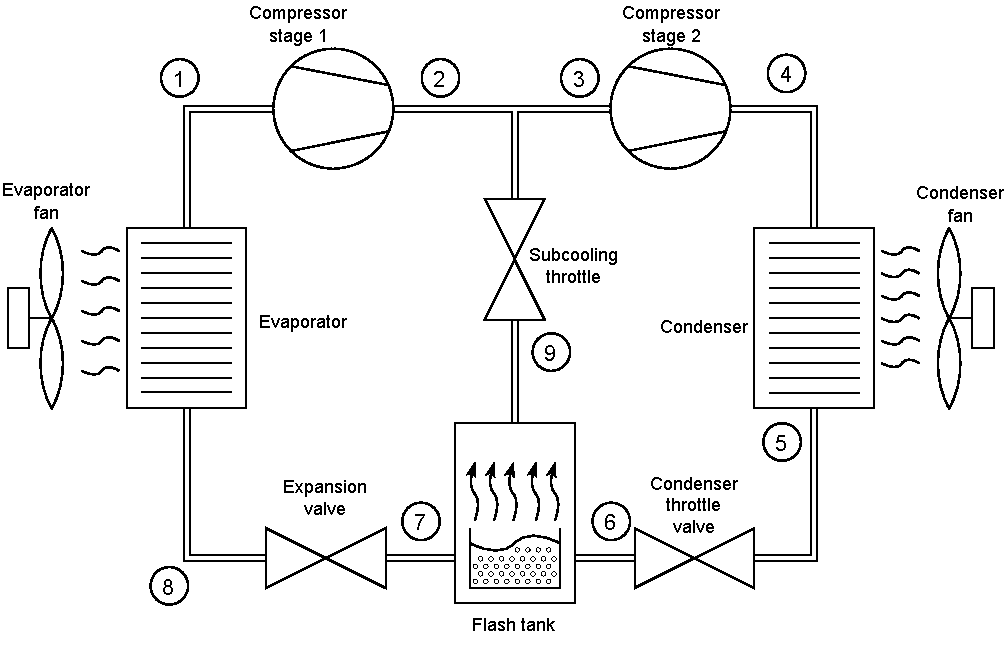
\includegraphics[width=0.8\textwidth]{Graphics/HVAC_Diagram_Fans.pdf}
	\caption{Illustration of refrigeration circuit}
	\label{fig:HVAC_Diagram}
\end{figure}
\todo{Missing reciever?}





\subsection{What is it used for}
	Lastbil
	
	
Inputs / outputs

Control objectives

	Const temp
		Disturbances
	Minimum energy consumption
		Prices of electricity and batteries are high
		
